\documentclass[10pt,twocolumn]{article}
\usepackage{amsmath}
\usepackage{amsfonts}
\usepackage{graphicx}
\usepackage{mathtools}
\usepackage{fullpage}
\usepackage{float}
\usepackage{color, soul}

\begin{document}
\title{6.867 HW2: Binary Classification Methods}
\maketitle
When making predictions and models, sometimes we would rather have discrete labels instead of continuous values. For example, if we were looking exam results, we might only care if students pass or fail. Alternatively, we may want to study electricity patterns, and at any given time lights can either be on or off. This idea of discrete labels is known as classification and in the case that there are only two options, binary classification. For the following work, we will consider the class labels $\{-1, +1\}$. 

\section{Logistic Regression}
 
 The first method we will use to implement binary classification will be logistic regression. The use of logistic functions, specifically the sigmoid, allow us to map continuous values of input values to a corresponding probability between 0 and 1, which then can be used to select a discrete label. Considering the maximum likelihood estimation, logistic regression can be written as 
 \begin{equation}
 \textrm{MLE}(w)= \sum_{i=1}^{n} \textrm{log}(1+e^{-y^{(i)}w^T \Phi(x^{(i)})})
 \end{equation}
 Where $w$ are the weights defining our model, $x(i), y(i)$ given data points, and $\Phi$ the basis functions from which we construct our model. Letting the basis function be a simple linear formulation, $\Phi(x)= \begin{bmatrix} 1 & x _1 & x_2 & ... \end{bmatrix}^T$, the above equation can be simplified as 
 \begin{equation}
\textrm{ NNL}(w)= \sum_{i=1}^{n}\textrm{ log}(1+e^{-y^{(i)}(w_0+w^Tx^{(i)})})
 \end{equation}
 However to prevent overfitting, we also want to introduce a regularization term into the logistic regression error function. Specifically we will consider a quadratic regularizer, which results in the finalized error function, 
 \begin{equation}
 E_{LR}(w)= \textrm{NNL}(w) +\lambda w^Tw
 \end{equation}
 Unlike some of the regression formulations we looked at last time, such as ridge or linear, there is no closed from solution to minimizing the error. Thus, we must employ optimization methods to select the correct weights. As far as optimization methods, two options are considered below, a simple gradient descent and the built in MATLAB optimization, fminunc. 
 
 Once weights are calculated from minimizing the error on the training data our classifier is simply defined as, 
 \begin{equation}
 h=\textrm{sign}(w^Tx +w_0)
 \end{equation}
 Which simply creates a hyperplane in which for any input, $x$. This classification returns -1 if $w^Tx+w_0<0$ and +1 if $w^Tx\geq 0$. The boundary decision is marked by $.5= \sigma (w^Tx)$ and is shown below for the case where there is no regularizer. 
 

 
 \begin{figure}[H]
\center
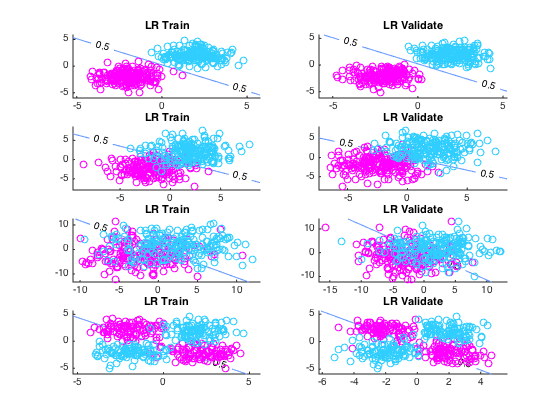
\includegraphics[scale =.4]{p1lambda0.png}
\caption{Labelled test and validation data for stdev1,stdev2, stdev4 and nonsep data sets. Also shown is the decision boundary }
\end{figure}
 
 Also considered was the error from mislabelled points, which was calculated for both the test and validation sets. Of course, the more easily separable the data, the lower the error. These results are shown in Table \ref{LR error}

As the magnitude of w increases the steepness of the hyperplane increases.  If $w$ goes to $ \infty$ the separator becomes a step function. The regularizer helps to limit this by penalizing the magnitude of the weights. It also helps prevent overfitting. So as $\lambda$ is increased the training error might increase since the cost is less influenced on the data error, NLL, and more influenced by the weights. 


We tested this logistic regression for $\lambda= \{0, 10, 1000\}$ and for the clearly separable and non separable case, there was no effect. For the stdev2, and stdev4 cases the training error increases but the validation error decreases. These results are shown in Table \ref{LR error}

 \begin{table}
 \caption{ Training and Validation Errors for different regularizers, $\lambda$}
  \begin{tabular}{ | c | c | c | c |}
 \hline
 dataset &$ \lambda=0 $& $\lambda=10$ & $\lambda=1000$ \\ \hline 
 stdev1 & [0,0] & [0,0] & [0,0] \\ \hline
 stdev2 & [36, 29] & [36,30] & [41, 26] \\ \hline
 stdev4 & [105, 99] & [105, 99] & [106, 98] \\ \hline 
 nonsep & [239, 247] & [243, 247] & [233, 228] \\ \hline
 \end{tabular}
 \label{LR error}
\end{table}
 
 
 
 \section{Support Vector Machine}
 
 Another implementation method of binary classification is the Support Vector Machine. In this classification method, we seek to divide the data into the different classifications with a clear a gap as possible. This gap or margin is defined as support vectors and takes advantage of the hinge loss.  The simplest form of SVM, the primal hard form, is expressed as 

 \begin{equation}
\min_w ||w||^2
\end{equation}
\begin{equation}
s.t. \: \forall i, y^{(i)}w^T x^{(i)} \geq 1 
 \end{equation}
    
 The hard form of SVM does not allow any leeway on the constraints, making it impossible to create a model if the data is not linearly separable. To increase the capability of the SVM, the soft SVM, includes a slack variable, $\xi$, For the straight forward primal form of soft SVM applied to the linear case,  $\Phi(x)= \begin{bmatrix} 1 & x _1 & x_2 & ... \end{bmatrix}^T$ , the overall objective once combined with corresponding constraint is thus
 \begin{equation}
 \min_{w, w_0} (\frac{1}{2} ||w||^2 + C \sum_{i=1}^n \xi_i)
 \end{equation}
 \begin{equation}
 s.t. \: y^{(i)}(w^Tx^{(i)} + w_0) \geq 1 -\xi_i
 \end{equation}   
 \begin{equation}
 \xi_i \geq 0
 \end{equation}
    
    
This formulation is not ideal, instead we translate this to the dual form which using an auxiliary variable, $\alpha$ to rewrite the SVM as a maximization and clearly shows the optimization as a maximum margin. 

\begin{equation}
\max_{\alpha \in \mathbb{R}^n} ( \sum_{i=1}^n \alpha_i - \frac{1}{2} \sum_{i=1}^n \sum_{j=1}^n \alpha_i \alpha_j y^{(i)} y^{(j)} (x^{(i)})^T x^{(j)})
\end{equation}
\begin{equation}
s.t. \: 0 \leq \alpha_i \leq C
\end{equation}
\begin{equation}
\sum_{i=1}^n \alpha_i y^{(i)} =0
\end{equation}

Instead of optimizing over the weights explicitly, we optimize over $\alpha$ from which the weights can be directly calculated as 
\begin{equation}
w= \sum_{i=1}^n \alpha_i y^{(i)}x^{(i)}
\end{equation}  
\begin{equation}
w_0= \frac{1}{M} ( \sum_{j \in M} y^{(j)} - \sum_{i \in S} \alpha_i y^{(i)}(x^{(j)})^Tx^{(i)})
\end{equation}

Where $S$ is the set of support vectors, $S=\{i : 0 < \alpha_i \leq C \}$ and $M = \{i : 0 < \alpha_i < C \}$. However since there is some numerical residual resulting from the optimizations of $\alpha$ that won't exactly equal 0 or C we will consider the small tolerance, $\epsilon= 10^-5$ so that  $S=\{i : \epsilon < \alpha_i \leq C-\epsilon \}$ and the same for M

\subsection*{Kernels}
      
\end{document}
